\section{Literatūros apžvalga}

Panaši problema į aptartąją įvade yra nemažai tyrinėjama duomenų bazių kontekste.
Čia minimizuojamas disko operacijų skaičius siekiant sumažinti duomenų bazės atsako laiką bei padidinti pralaidumą (apdorotų užklausų skaičių per laiko vienetą) \cite{garcia2000database}.
Panašiai kaip šiame darbe siekiama minimizuoti biometrinių įrašų blokų skaičių likusį po atmetimo etapo siekiant pagerinti sistemos \cite{NeurotechnologyMegamatcherAccelerator} pralaidumą.
Tuo tikslu yra naudojama duomenų struktūra, vadinama {\it duomenų indeksu}.
Jeigu duomenys yra daugiamačiai (vienas įrašas gali susidėti iš daugiau negu vienos reikšmės), tuomet indeksas tokiems duomenims vadinamas {\it daugiamačių duomenų indeksu}, o metodas pagal kurį šis indeksas yra sudaromas bei naudojamas {\it daugiamačių duomenų indeksavimo metodu}.

\subsection{Užklausų klasifikacija}

Šiame darbe palyginant indeksavimo metodus sistemoje \cite{NeurotechnologyMegamatcherAccelerator} siekiama apimti kiek galima daugiau užklausų klasių pagal Gaede ir Günther \cite{gaede1998multidimensional} pateikiamą daugiamačių užklausų klasifikaciją:
\begin{enumerate}
	\item Griežto atitikmens užklausa
	\item Taško užklausa
	\item Lango užklausa
	\item Regiono užklausa
	\item Apgaubiančioji užklausa
	\item Pilno regiono užklausa
	\item Kaimynų užklausa
	\item Artimiausio kaimyno užklausa
\end{enumerate}

Autorius duomenis ir užklausas nagrinėja $d$ dimensijų euklido erdvėje $E^d$.
Atskirus įrašus apibrėžia kaip objektus $o$ kurie gali turėti 0 ar daugiau papildomų atributų nesusijusių su erdve $E^d$ (pvz.: vardas, pavadinimas, amžius...), bei griežtai vieną atributą $o.G$, kuris apibūdina objekto $o$ padėtį erdvėje $E^d$.
Šis $o.G$ atributas yra aibė taškų, kuriuos objektas $o$ užima erdvėje $E^d$.
Objektams yra apibrėžiami operatoriai $=$, $\cap$, bei $dist(o_1, o_2)$.
Du objektai $o_1$ ir $o_2$ skaitomi lygiais $o_1 = o_2$ tada ir tik tada jeigu abiejų objektų užimamų taškų aibės $o_1.G$ ir $o_2.G$ sutampa.
Dviejų objektų $o_1$ ir $o_2$ sankirta $o_1 \cap o_2$ yra aibė taškų, kurie patenka ir į $o_1.G$ ir į $o_2.G$.
Ir galiausiai atstumas tarp dviejų objektų $o_1$ ir $o_2$ $dist(o_1, o_2)$ skaitomas mažiausias atstumas tarp bet kurių dviejų taškų esančių $o_1.G$ ir $o_2.G$ aibėse.



\subsubsection{Griežto atitikmens užklausa}
Griežto atitikmens užklausa yra tokia užklausa, kuri duotąjam objektui $o'$ erdvėje $E^d$ randa visus objektus, kurių erdvės sritys sutampa su duotąja:

\begin{equation}
	EMQ(g) = \{ o | o'.G = o.G \}
\label{eq:ExactMatchQuery}
\end{equation}

\subsubsection{Taško užklausa}
Taško užklausa yra tokia užklausa, kuri duotam taškui $p$ erdvėje $E^d$ randa visus objektus, kurie turi bendrų taškų:

\begin{equation}
	PQ(p) = \{ o | \{p\} \cap o.G = \{p\} \}
\label{eq:ExactMatchQuery}
\end{equation}

Žiūrėti priedą \ref{app:pointQuery}.

\subsubsection{Lango užklausa}
Lango užklausa, tai tokia užkausa, kuri duotiems $d$ intervalams $I^d = [l_1, u_1] \times [l_2, u_2] \times ... \times [l_d, u_d]$ (po vieną kiekvienai erdvės $E^d$ koordinačių ašiai) randa visus objektus $o$ kurie turi bendrų taškų:

\begin{equation}
	WQ(I^d) = \{ o | I^d \cap o.G \neq \emptyset \}
\label{eq:ExactMatchQuery}
\end{equation}

Verta pastebėti, kad lango užklausos atveju visos erdvės srities kraštinės yra lygegriačios erdvės $E^d$ koordinačių ašims.
Žiūrėti priedą \ref{app:windowQuery}.


\subsubsection{Regiono užklausa}
Regiono užklausa yra labai panaši į Lango užklausą, tačiau srities kraštinės gali būti laisvai pasirinktos, ir neturi būti lygegriačios koordinačių ašims.
Regiono užklausa randa visus objektus, kurie turi bendrų taškų su duotuoju objektu $o'$.

\begin{equation}
	IQ(g) = \{ o | o'.G \cap o.G \neq \emptyset \}
\label{eq:ExactMatchQuery}
\end{equation}
Žiūrėti priedą \ref{app:intersectionQuery}.

\subsubsection{Apgaubiančioji užklausa}
Apgaubiančioji užklausa yra tokia užklausa, kuri randa visus objektus $o$, kurių erdvės sritis $o.G$ pilnai apima pateiktąjį objektą $o'$:

\begin{equation}
	EQ(g) = \{ o | (o'.G \cap o.G) = o.G \}
\label{eq:ExactMatchQuery}
\end{equation}
Žiūrėti priedą \ref{app:enclosureQuery}.


\subsubsection{Pilno regiono užklausa}
Pilno regiono užklausa iš esmės yra priešinga apgaubiančiąjai.
Pilno regiono užklausa yra tokia užklausa, kuri randa visus objektus $o$, kurių erdvės sritis $o.G$ pilnai patenka į pateikatjį objektą $o'$:

\begin{equation}
	CQ(g) = \{ o | (o'.G \cap o.G) = o'.G \}
\label{eq:ExactMatchQuery}
\end{equation}
Žiūrėti priedą \ref{app:containmentQuery}.


\subsubsection{Kaimynų užklausa}
Kaimynų užklausa yra tokia užklausa, kuri pagal duotąjį objektą $o'$ suranda visus šio objekto kaimynus, t.y. objektus $o$ kurie turi bendrą kraštinę erdvėje $E^d$:

\begin{equation}
	AQ(g) = \{ o | (o'.G \cap o.G) \neq \emptyset \land o'.G\textdegree \cap o.G\textdegree = \emptyset \}
\label{eq:ExactMatchQuery}
\end{equation}

Čia $o.G\textdegree$ reiškia visus vidinius taškus, kurie priklauso sričiai $o.G$.
Žiūrėti priedą \ref{app:adjacencyQuery}.


\subsubsection{Artimiausio kaimyno užklausa}
Artimiausio kaimyno užklausa yra tokia užklausa, kuri duotam objektui $o'$ randa artimiausią kaimyną (verta pastebėti, kad šiuo atveju kaimynai gali ir neturėti bendrų kraštinių).

\begin{equation}
	NNQ(o') = \{ o | \forall o'' : dist(o'.G, o.G) \leq dist(o'.G, o''.G) \}
\label{eq:ExactMatchQuery}
\end{equation}




\subsection{Daugiamačių duomenų indeksavimo metodų klasifikacija}
Lu ir Ooi \cite{lu1993spatial}, Gaede ir Günther \cite{gaede1998multidimensional}, bei B{\"o}hm, Christian, Stefan, Daniel A \cite{bohm2001searching} apžvelgia įvairius daugiamačių duomenų indeksus, bei pateikia schemą padedančią suprasti jų istoriją (žiūrėti priedą \ref{app:multidimensionalIndexing}).

Autoriai šiuos metodus suskirsto į tris grupes:
\begin{itemize}
	\item Metodai paremti maišos funkcijomis.
	\item Hierarchiniai metodai.
	\item Metodai paremti erdvę užpildančiomis kreivėmis \cite{bader2012space}.
\end{itemize}



\subsubsection{Maišos funkcijomis paremti metodai daugiamačių duomenų indeksavimui}

Bendruoju atveju maišos funkcijomis paremti metodai yra tinkami griežto atitinkmens, bei taško užklausoms.
Tačiau siekiant apdoroti lango, regiono ir kitas, panašias, užklausias šie metodai tampa kompleksiškesni \cite{nievergelt1981grid} \cite{tamminen1982excell}.
Dėl šios priežasties jie nebus nagrinėjami, įgyvendinami ir lyginami šiame darbe.


\subsubsection{Hierarchiniai metodai daugiamačių duomenų indeksavimui}

Hierarchiniai daugiamačių duomenų indeksai yra paremti dvejetainiais ar aukštesnio atsišakojimo faktoriaus medžiais (trejetainiai, ketvirtainiai...) \cite{gaede1998multidimensional}.
Šie indeksai saugo įrašus ne po vieną, bet grupėmis.
Dažniausiai kiekviena grupė yra randama medžio lapuose (vadinama {\it duomenų viršūne}).
Vidinės viršūnės (vadinamos {\it indekso viršūnėmis}) yra naudojamos kaip kelrodžiai ieškant duomenų viršūnių.
Kiekviena indekso viršūnė nurodo visas duomenų viršūnes, kurios gali būti rastos šios indekso viršūnės pomedyje.

%TODO: image

Užklausų apdorojimas yra skaidomas į du etapus:
\begin{enumerate}
	\item Iteravimas medžiu.
	\item Įrašų filtravimas.
\end{enumerate}
Iteravimo medžiu etape, yra „prabėgamas“ medis nuo šaknies iki lapų ir atrenkamos visos duomenų viršūnės, kurios gali turėti įrašų atitinkančių užklausą.
Filtravimo metu atrenkami įrašai esantys iteravimo etape atrinktose grupėse ir tenkinatys užklausą \cite{brinkhoff1994multi} \cite{bohm2001searching}.
Verta pastebėti, kad sistemoje \cite{NeurotechnologyMegamatcherAccelerator} užklausų apdorojimo etapai yra labai panašūs.

\paragraph{Kd-medis}

Šiame darbe bus aptariamas biometrinių įrašų priskyrimo blokams metodas paremtas Kd-medžiu \cite{bentley1979multidimensional}.
Kd-medžių duomenys yra taškai $E^d$ erdvėje.
Kd-medis yra dvejetainis medis, kurio lapuose (duomenų viršūnėse) yra saugomi vienas ar daugiau $d$-mačių taškų.
Kiekviena vidinė medžio viršūnė (indekso viršūnė) dalina erdvę $E^d$ į dvi nepersidengiančias dalis.
Taškai patenkantys į vieną dalį patenka į kairyjį pomedį, o patenkantis į kitą dalį -- į dešinį pomedį (žr.: \ref{img:KdTreeExample} pav.).
Erdvės dalinimas į dvi dalis yra parenkamas taip: kiekvienai vidinei viršūnei yra parenkama koordinačių ašis (pvz.: $x$) ir reikšmė (pvz .: $5$).
Tuomet visi taškai, kurių $x$ koordinatės reikšmė yra mažesnė už parinktą reikšmę (pavyzdyje $[-\infty; 5)$), patenka į kairyjį pomedį, likę taškai (pavyzdyje $[5; \infty)$) -- į dešinį pomedį.
Nėra griežtai apibrėžta kokia koordinačių ašis ar reikšmė šioje ašyje turi būti parinkta kiekvienai viršūnei, todėl šiuo tikslu taikomos įvairios euristikos.

\begin{figure}[H]
\begin{center}
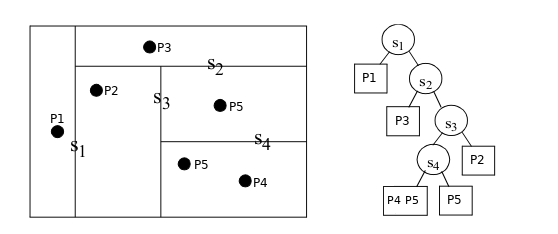
\includegraphics[width=0.7\textwidth]{img/KdTreeExample.png}
\caption{Kd-medžio pavyzdys.}
\label{img:KdTreeExample}
\end{center}
\end{figure}

Paveiksliuke \ref{img:KdTreeExample} pateikiamas Kd-medžio pavyzdys.
Čia kairėje -- šį medį atitinkanti erdvė $E^d$.
Taškai $P1$-$P5$ atitinka daugiamačius duomenis, o tiesės $S1$-$S4$ - erdvės $E^d$ padalijimus atitinkmai medžio viršūnėse $S1$ - $S4$.

Hierarchiniai metodai daugiamačių duomenų indeksavimui yra plačiai taikomi duomenų bazių \cite{bohm2001searching}, sensorių tinklų \cite{li2003multi}, paveiksliukų paieškoje \cite{silpa2008optimised}, privatumo \cite{hore2012secure} \cite{xiao2010differentially} ir kitose srityse.

\subsubsection{Erdvę užpildančiomis kreivėmis paremti metodai daugiamačių duomenų indeksavimui}

Kaip ir hierarchiniuose metoduose taip ir erdvę užpildančiomis kreivėmis paremtuose metoduose duomenys nagrinėjami kaip taškai euklido erdvėje $E^d$.

Daugiamačiai duomenys neturi pilnos tvarkos, pagal kurią šalia esantys taškai būtų arti ir erdvėje $E^d$.
Dėl šios priežasties daugiamačių duomenų indeksavimo metodai yra sudėtingesni lyginant su vienmačiais \cite{gaede1998multidimensional} \cite{bohm2001searching}
Tačiau egzistuoja įvairiomis euristikomis paremtų pilnos tvarkos sudarymo metodų, kurie su nemaža tikimybe taip sudeda taškus.
Ši pilna tvarka yra vienmatė erdvė $E'^1$ kurią galima indeksuoti vienmačiais indeksavimo metodais (B-medžiu \cite{comer1979ubiquitous} RB-medžiu \cite{hanke1997relaxed} ir pan.).

Siekiant sudaryti tokią tvarką, $E^d$ erdvė suskirstoma į gardelę (į kiekvieną laukelį šioje gardelėje gali patekti nulis, vienas ar daugiau taškų).
Kiekvienam laukeliui šioje gardelėje yra priskiriamas unikalus skaičius pagal kurį laukeliai yra surikiuojami ir indeksuojami vienmačiais indeksavimo metodais.
Šie unikalūs skaičiai yra priskiriami pagal tai kokia tvarka erdvę užpildanti kreivė \cite{bader2012space} „prabėga“ pro laukelius.
Aptarsime dvi tokias kreives:
\begin{enumerate}
	\item Eilutinę kreivę.
	\item Z-kreivę.
\end{enumerate}

\paragraph{Eilutinė kreivė}

Eilutinė kreivė yra viena iš papraščiausių erdvę užpildančių kreivių.
Ji negali būti naudojama begalinėje erdvėje, todėl tarkime, kad $[L_i; U_i]$ yra erdvės $E^d$ ribos dimensijos $i$ atžvilgiu.
Eilutinė kreivė iš pradžių „prabėga“ visus taškus didėjimo tvarka $[x, L_2, ..., L_d]$, kur $x \in [L_1; U_1]$.
Paskui „prabėga“ $[x, L_2 + 1, ..., L_d]$, paskui $[x, L_2 + 2, ..., L_d]$ ir t.t. (žr.: \ref{img:RowWiseSpaceFillingCurve} pav.).

\begin{figure}[H]
\begin{center}
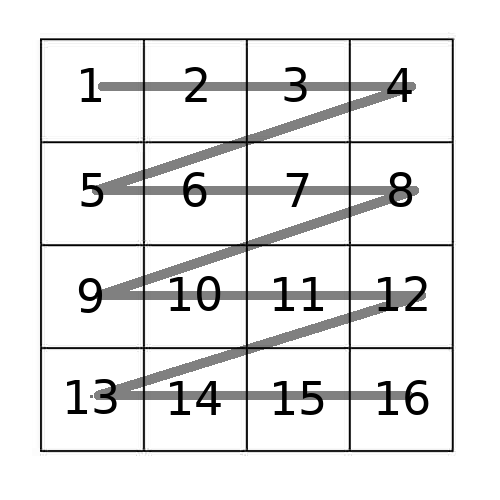
\includegraphics[width=0.3\textwidth]{img/RowWiseSpaceFillingCurve.png}
\caption{Eilutinės erdvę užpildančios kreivės pavyzdys.}
\label{img:RowWiseSpaceFillingCurve}
\end{center}
\end{figure}


Formaliai tvarka yra apibrėžiama sąryšio:
\begin{equation}
	p_1 < p_2 \text{ jeigu } RWSFC(p_1) < RWSFC(p_2)
\label{eq:RowWiseSFCComparison}
\end{equation}

Čia $p_1$ ir $p_2$ yra taškai erdvėje $E^d$, o $RWSFC(p)$:

\begin{equation}
	RWSFC(p) = 1 + \sum_{i=1}^{d} [(p_i - L_i) \prod_{j=0}^{i - 1}U_j - L_j]
\label{eq:RowWiseSFCValue}
\end{equation}

Čia daroma prielaida, kad $U_0 - L_0 = 1$.



\paragraph{Z-kreivė}

Daugiamačių duomenų indeksavimo metodų paremtų erdvę užpildančiomis kreivėmis kontekste Z-kreivė yra viena iš populiariausių \cite{ramsak2000integrating}.
Z-kreivė visų pirmą visą erdvę $E^d$ padalina į dvi lygias sritis $p_0$ ir $p_1$ statmenai pirmai koordinačių ašiai.
Z-kreivė visus laukelius esančius srityje $p_0$ „prabėga“ pirmiau tų, kurie yra srityje $p_1$.
Sekančiame žingsnyje $p_0$ ir $p_1$ yra padalinamos į dvi lygias sritis $p_{00}$, $p_{01}$ bei $p_{10}$ $p_{11}$ statmenai antrai koordinačių ašiai.
Atitinkamai $p_{00}$ laukeliai yra „prabėgami“ ankščiau $p_{01}$, o $p_{10}$ ankščiau $p_{11}$.
Toliau skaidoma pagal trečią koordinačių ašį, vėliau pagal ketvirtą, ..., d-tąją (žr.: \ref{img:ZCurveSpaceFillingCurve} pav.).
Kai padaromas padalinimas pagal d-tąją ašį, pradedama vėl nuo pirmosios koordinačių ašies.
Šis rekursiškas dalinimas yra vykdomas tol, kol kiekviena erdvės sritis $p$ yra nedidesnė negu ankščiau minėtos gardelės laukelio dydis.

\begin{figure}[H]
\begin{center}
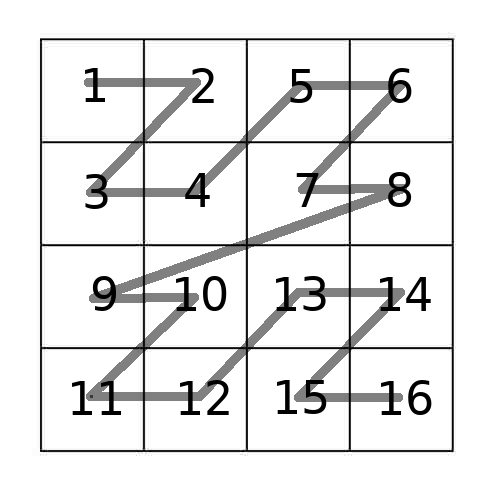
\includegraphics[width=0.3\textwidth]{img/ZCurveSpaceFillingCurve.png}
\caption{Z erdvę užpildančios kreivės pavyzdys.}
\label{img:ZCurveSpaceFillingCurve}
\end{center}
\end{figure}

Tarsime, kad erdvė $E^d$ nėra begalinė, ir $[0, 2^b]$ yra visų šios erdvės koordinačių ašių ribos.
Formaliai tvarka yra apibrėžiama sąryšio:
\begin{equation}
	p_1 < p_2 \text{ jeigu } ZCSFC(p_1) < ZCSFC(p_2)
\label{eq:ZCurveSFCComparison}
\end{equation}

Čia $p_1$ ir $p_2$ yra taškai erdvėje $E^d$, o $ZCSFC(p)$:

\begin{equation}
	ZCSFC(p) = \sum_{i=0}^{b-1} \sum_{j=0}^{d-1} [2^{i*b+j} BITSET(p_j, i)]
\label{eq:ZCurveSFCValue}
\end{equation}


\begin{equation}
	BITSET(p, i)=
\begin{cases}
	1,& \text{jeigu } \text{i-asis bitas yra 1 skaičiaus p dvejetainėje formoje}\\
	0,& \text{kitu atveju}\\
\end{cases}
\label{eq:Bitset}
\end{equation}






\subsection{SP-GIST karkasas}
% sp-gists
% bulk operations on sp-gists
% postgre (min 3)
